\section{The Op Vocabulary Gap}
\label{sec:transfer}
\label{sec:op_gap}

We test whether the gaps we measure reduce to training-data coverage with a matched-compute SFT ablation on a Qwen2-VL-2B backbone (9 GPU-hour budget, 162K samples per variant): (\textbf{A}) sketch+extrude only, mirroring CAD-Recode; (\textbf{B}) 50/50 mixture of A and BenchCAD-Synth; (\textbf{C}) BenchCAD-Synth + GenCAD only. Table~\ref{tab:op_gap} shows variant A scores \textbf{0\% recall on every essential operation} (helix, sweep, loft, twist-extrude, parametric involute-gear construction) --- not because the underlying Qwen2-VL lacks the API vocabulary, but because its SFT distribution never demonstrates these operations. We name this systematic deficit the \textbf{Op Vocabulary Gap}. Variant B recovers 22--35 points of essential-op recall while losing only 5\,pt on DeepCAD IoU; variant C recovers further (35--48\%) at 45\,pt cost on legacy IID. A complementary transfer of the released CAD-Recode/cadrille/CADEvolve checkpoints~\citep{Rukhovich2025,Kolodiazhnyi2026,Elistratov2026} loses 28--32\,pt on BenchCAD-Lite despite $>$90\% IoU on their own benchmarks (Table~\ref{tab:transfer}; full cadrille-vs-CADEvolve breakdown in Appendix~\ref{app:transfer_detail}).

\begin{table}[t]
    \centering
    \small
    \setlength{\tabcolsep}{4pt}
    \caption{\textbf{TODO Per-operation recall on Vision2Code} with paired comparison of gpt-5.3 (chat-latest) vs gpt-5.3-thinking.              
    Thinking-mode degrades both macro recall (advanced: 25.2 → 22.8, all: 35.1 → 32.3) and execution rate (69.5 → 
    67.5), against the common expectation that inference-time reasoning monotonically helps. Looking inside the per-op 
    deltas reveals a structural trade: thinking improves recall on composition-choice and finishing operations that 
    benefit from explicit planning (loft +17.6, polygon +18.2, fillet +12.0, rarray +7.2) but degrades on direct       
    boolean and scaffolding operations (cut −11.9, cutBlind −10.5, workplane −8.9, sweep −7.7, box −7.7, union −5.6). 
    The net effect is a synthesis-execution trade-off
    — the model thinks more about which high-level op
    to call, while writing the surrounding boilerplate
    less reliably.}
    \label{tab:op_recall}
  \begin{tabular}{lrrr}                                             
  \toprule                                                                                 
  Operation & gpt-5.3 & gpt-5.3-thk & $|\text{GT}|$ \\                                                             
  \midrule                                                                                                             
  \multicolumn{4}{l}{\emph{Basic ops (shared with prior corpora: cad-recode / text2cad)}} \\                           
  \texttt{extrude}              & 83.3          & \textbf{84.4} & 90  \\                                               
  \texttt{cut}                  & \textbf{44.1} & 32.2          & 59  \\                                               
  \texttt{union}                & \textbf{65.3} & 59.7          & 72  \\                                               
  \texttt{circle}               & \textbf{78.7} & 77.3          & 75  \\                                               
  \texttt{cylinder}             & 4.5           & \textbf{7.6}  & 66  \\                                               
  \texttt{box}                  & \textbf{42.3} & 34.6          & 78  \\                                               
  \texttt{rect}                 & 63.0          & \textbf{65.2} & 46  \\                                               
  \texttt{workplane}            & \textbf{86.3} & 77.4          & 124 \\                                               
  \midrule                                                                                                             
  \multicolumn{4}{l}{\emph{Advanced ops (BenchCAD-distinguishing)}} \\                                                 
  \texttt{hole}                 & \textbf{60.2} & 55.4          & 83  \\                                               
  \texttt{chamfer}              & \textbf{8.6}  & 4.3           & 70  \\                                               
  \texttt{cutThruAll}           & \textbf{16.2} & 10.8          & 37  \\                                               
  \texttt{revolve}              & \textbf{14.3} & 10.7          & 28  \\                                               
  \texttt{fillet}               & 0.0           & \textbf{12.0} & 25  \\
  \texttt{cutBlind}             & \textbf{36.8} & 26.3          & 19  \\                                               
  \textbf{\texttt{loft}}        & 5.9           & \textbf{23.5} & 17  \\
  \texttt{threePointArc}        & \textbf{6.2}  & 0.0           & 16  \\                                               
  \texttt{rarray}               & 7.1           & \textbf{14.3} & 14  \\                                               
  \textbf{\texttt{sweep}}       & \textbf{53.8} & 46.2          & 13  \\                                               
  \texttt{polygon}              & 54.5          & \textbf{72.7} & 11  \\                                               
  \texttt{makeHelix}            & 12.5          & 12.5          & 8   \\                                               
  \texttt{slot2D}               & 25.0          & 25.0          & 8   \\                                               
  \texttt{polarArray}           & 20.0          & 20.0          & 5   \\                                               
  \texttt{shell}                & \textbf{25.0} & 0.0           & 4   \\
  \texttt{mirrorY}              & 0.0           & 0.0           & 4   \\                                               
  \texttt{sphere}               & 100.0         & 100.0         & 4   \\
  \texttt{cboreHole}            & 0.0           & 0.0           & 3   \\                                               
  \texttt{radiusArc}            & \textbf{33.3} & 0.0           & 3   \\
  \midrule                                                                                                             
  \textbf{Macro recall} (advanced, 19 ops) & \textbf{25.2\%} & 22.8\% & --- \\
  \textbf{Macro recall} (all, 27 ops)      & \textbf{35.1\%} & 32.3\% & --- \\                                         
  \textbf{Exec rate}                       & \textbf{69.5\%} & 67.5\% & --- \\                                         
  \bottomrule                                                                                                          
  \end{tabular}                                                                                                       
                                     
    % \begin{tabular}{lrrrr}
    % \toprule
    % Operation & baseline & ood & iid & $|\text{GT}|/100$ \\
    % \midrule
    % \multicolumn{5}{l}{\emph{Basic ops (shared with prior corpora: cad-recode / text2cad)}} \\
    % \texttt{extrude}              & 100.0 & 91.7  & 95.8  & 24 \\
    % \texttt{cut}                  & 87.2  & 70.2  & 89.4  & 47 \\
    % \texttt{union}                & 91.7  & 41.7  & 79.2  & 24 \\
    % \texttt{circle}               & 82.8  & 79.3  & 96.6  & 29 \\
    % \texttt{cylinder}             & 5.9   & 88.2  & 94.1  & 17 \\
    % \texttt{box}                  & 2.6   & 84.6  & 92.3  & 39 \\
    % \texttt{rect}                 & 5.0   & 65.0  & 90.0  & 20 \\
    % \texttt{workplane}            & 0.0   & 77.4  & 88.7  & 53 \\
    % \midrule
    % \multicolumn{5}{l}{\emph{Advanced ops (BenchCAD-distinguishing)}} \\
    % \textbf{\texttt{revolve}}     & \textbf{0.0} & \textbf{54.8} & \textbf{93.5} & 31 \\
    % \textbf{\texttt{loft}}        & \textbf{0.0} & \textbf{22.2} & \textbf{77.8} &  9 \\
    % \textbf{\texttt{sweep}}       & \textbf{0.0} & \textbf{25.0} & \textbf{75.0} &  8 \\
    % \textbf{\texttt{sweep+helix}} & \textbf{0.0} & \textbf{100.0}& \textbf{50.0} &  2 \\
    % \textbf{\texttt{twistExtrude}}& \textbf{0.0} & \textbf{100.0}& \textbf{100.0}&  1 \\
    % \texttt{fillet}               & 0.0   & 25.0  & 87.5  &  8 \\
    % \texttt{chamfer}              & 0.0   & 85.3  & 85.3  & 34 \\
    % \texttt{shell}                & 0.0   & 80.0  & 100.0 &  5 \\
    % \texttt{hole}                 & 0.0   & 82.8  & 93.1  & 29 \\
    % \texttt{rarray}               & 0.0   & 77.8  & 100.0 &  9 \\
    % \texttt{polarArray}           & 0.0   & 33.3  & 83.3  &  6 \\
    % \midrule
    % \textbf{Macro recall} (16 ops) & \textbf{17.5\%} & \textbf{59.9\%} & \textbf{84.0\%} & --- \\
    % \textbf{Exec rate}             & 90.0\% & 94.0\% & 99.0\%        & --- \\
    % \bottomrule
    % \end{tabular}
    \end{table}

    

\begin{table}[t]
\centering
\small
\caption{\textbf{Transfer of CAD-specialised SOTA models to BenchCAD-Lite.} Both cadrille-RL and CADEvolve match published numbers on the DeepCAD test split within $\pm$0.5\,pt under our scoring infrastructure but lose 28--32\,pt on BenchCAD's standard-anchored, operation-rich evaluation. Our open BenchCAD-trained baseline (Qwen2-VL-2B SFT-only) reproduces the lineage's training stack without RL and bounds dataset difficulty with a publicly auditable lower curve.}
\label{tab:transfer}
\begin{tabular}{lrr|rr}
\toprule
Model & DeepCAD IoU & Our DeepCAD & BenchCAD IoU & $\Delta$ \\
\midrule
cadrille-RL~\citep{Kolodiazhnyi2026}  & 92.2 & 91.9 & 60.5 & $-$31.4 \\
CADEvolve-rl1~\citep{Elistratov2026}  & 92.6 & 92.3 & 64.1 & $-$28.2 \\
\midrule
BenchCAD-trained baseline (ours, SFT-only) & 78.4 & 78.2 & 22.7 & $-$55.5 \\
\bottomrule
\end{tabular}
\end{table}


\begin{figure*}[t]
  \centering
  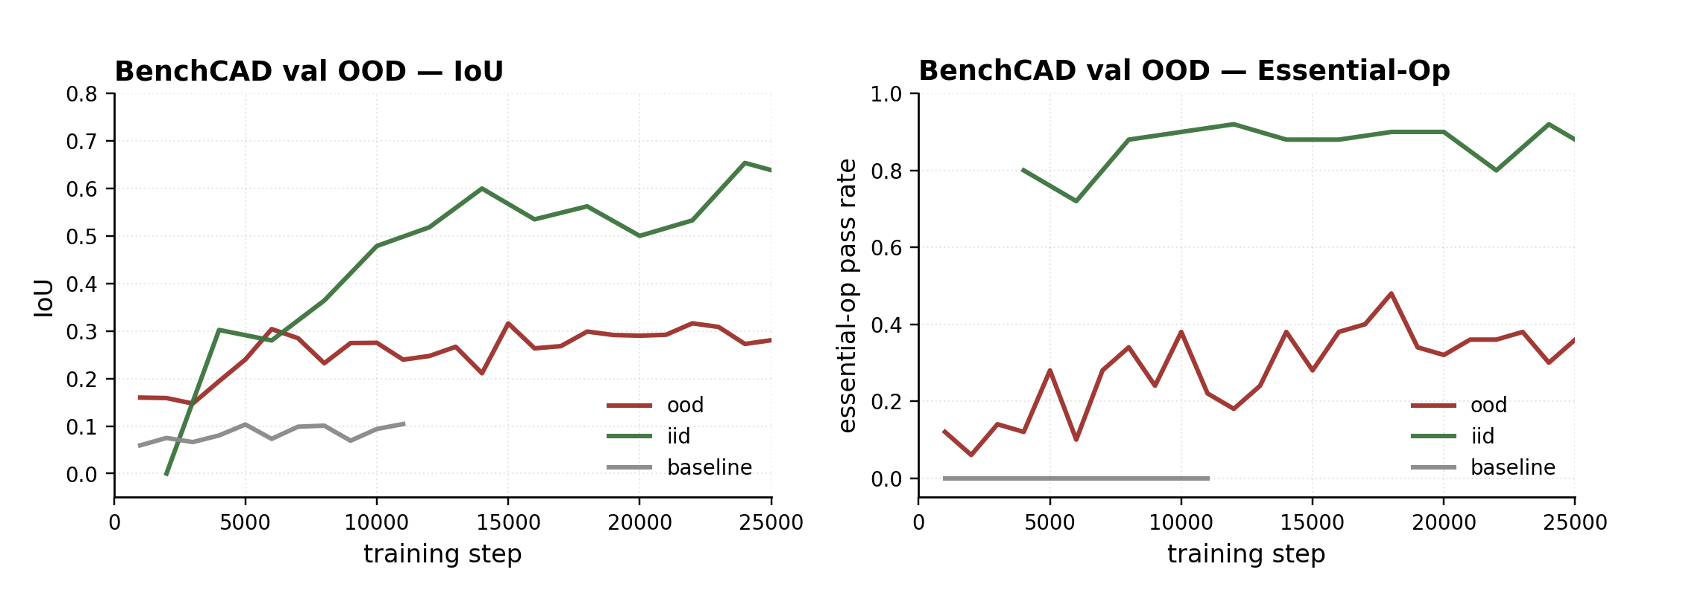
\includegraphics[width=0.75\linewidth]{figures/fig_7.png}
  \caption{\textbf{The generalisation gap on BenchCAD remains substantial after 25k SFT steps.} Qwen2-VL-2B trained on three data mixtures under matched 9 GPU-hour budgets, evaluated on the BenchCAD validation set throughout 0--25k steps.
    \emph{(a) OOD IoU vs.\ training step.} The IID-trained run (green) climbs to IoU $\sim$0.65; the OOD run (red, trained without the target family slice) plateaus near 0.30 by 10k steps; the HQ-only baseline (grey, no BenchCAD-Synth) never exceeds 0.10. \emph{(b) OOD essential-op pass rate.} IID reaches $\sim$0.85, OOD plateaus at $\sim$0.35, HQ-only stays at $\sim$0\% --- the \textbf{Op Vocabulary Gap}.
    The deficit is not optimisation budget (curves saturate by 15--20k), not backbone capacity (same Qwen2-VL-2B reaches IID IoU 0.65), and not training-corpus operation coverage alone (the OOD run \emph{has} BenchCAD-Synth data and still plateaus 35--50\,pt below IID). It is the fundamental difficulty of training large models to construct industry-grade parametric CAD code on \emph{unseen} family distributions.}
  \label{fig:generalisation_gap}
\end{figure*}
